\chapter{Cas d'utilisation}

Nous avons procédé à l'analyse de la méthode GTD et modélisé de manière très générale les différents acteurs et actions du système. Le diagramme suivant sera décomposé dans la suite en 4 sous-diagrammes de cas d'utilisation :\\


\begin{itemize}

\item Cas d'utilisation : Collecter des données
\item Cas d'utilisation : Traiter des données
\item Cas d'utilisation : Organiser des données
\item Cas d'utilisation : Réactuliser\\

\end{itemize}


La sélection des informations peut engendrer une création de tâches d'où la relation extend.
Le cas d'utilisation Revue doit permettre de collecter de nouvelles informations. En effet, lorsque de nouvelles tâches sont traitées, de nouvelles informations peuvent en découler.



\begin{figure}[H]
\begin{center}
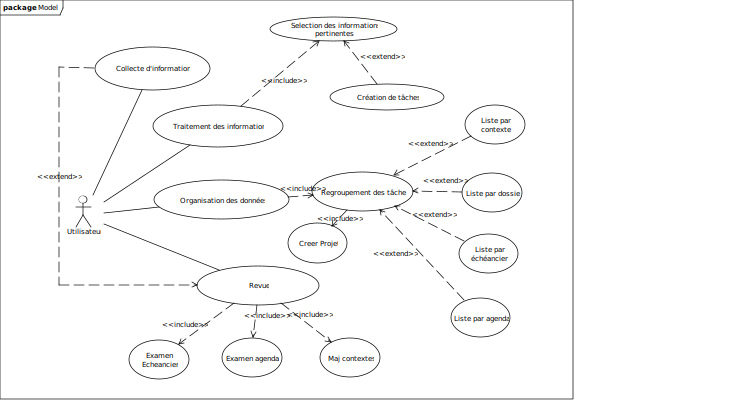
\includegraphics[scale=0.4,angle=90]{diagrams/UseCase.png}
\caption{Diagramme UML de cas d'utilisation - Vision générale du système}
\end{center}
\end{figure}





\section {Recensement des taches}
\subsection*{Cockburn du recensement des taches}
\begin{tabular}{|p{1.1in}|p{1.1in}|p{2.0in}|p{1.5in}|} \hline 
\textbf{Cas d'utilisation} & \multicolumn{3}{|p{3.2in}|}{Collecter des informations} \\ \hline 
\textbf{Acteur} & \multicolumn{3}{|p{3.2in}|}{Objectif Utilisateur} \\ \hline 
\textbf{Parties prenantes et intérêts} & \multicolumn{3}{|p{5in}|}{~Le recensement exhaustif 
de tout ce qui peut justifier une quelconque intervention de notre part : en suspens, 
inachèvement, en attente, intention, projet, manque, usure, mauvais fonctionnement, 
problème, insatisfaction, besoin, engagements à tenir,etc.\newline Exemples: cette 
carte de visite restée dans une poche, cette facture dans la boîte à gants, cette 
demande reçue, ce dossier qui traîne sur le bureau, cette agrafeuse qui coince, cette 
course à faire, ce problème à résoudre, cette suggestion à tester, les messages de 
la boîte vocale, ce projet jamais réalisé, ce souci de santé, ce fauteuil qui grince, 
les performances de ce collaborateur, toutes ces choses en retard...} \\ \hline 
\textbf{Niveau} & \multicolumn{3}{|p{3.2in}|}{~Utilisateur} \\ \hline 
\textbf{Portée} & \multicolumn{3}{|p{3.2in}|}{~Système 
GTD} \\ \hline 
\textbf{Pré-conditions} & \multicolumn{3}{|p{3.2in}|}{~} \\ \hline 
\textbf{Post-conditions} & \multicolumn{3}{|p{4.6in}|}{~Les informations sont enregistrées sur un support.} \\ \hline 
\textbf{Scénario nominal} & \textbf{Etapes} & \textbf{Action} & ~ \\ \hline 
~ & 1 & ~Recenser tout ce qui justifie une intervention de l'utilisateur~ & ~ \\ \hline 
 & 2 & Enregistrer les informations (postit, système d'information) &  \\ \hline 
\textbf{Extensions} & \textbf{Etapes} & \textbf{Condition} & \textbf{Action} \\ \hline 
~ & * & A 
tout moment & ~Possibilité d'annuler l'action \\ \hline 
\textbf{Contraintes} & \textbf{Type} & \textbf{Description} & ~ \\ \hline 
~ & ~Correction & ~Les informations ennoncées sont réelles et correct. & ~ \\ \hline 
\textbf{Priorité} & \multicolumn{3}{|p{3.2in}|}{~Elevée 
(5/5)} \\ \hline 
\textbf{Performance} & \multicolumn{3}{|p{3.2in}|}{~} \\ \hline 
\textbf{Fréquences} & \multicolumn{3}{|p{3.2in}|}{~Tous les débuts de journée} \\ \hline 
\end{tabular}



\subsection*{Scenario du recensement des taches}

	Le scénario du cas d'utilisation \textit{Collect} est très simple : Il correspond à un travail que doit fournir l'utilisateur. A savoir le recensement des informations sur tout ce qui peut nécessiter une intervention de notre part. La première partie concerne donc le rencensement puis une saisie est effectuée sur le système (post-it ou système informatique).
	
\subsection*{Diagramme d'objet}

\subsubsection {Avant \textit{le recensement des tâches}}

\begin{figure}[H]
	\begin{center}
	\includegraphics[scale=0.8]{diagrams/InstantaneCollectBefore.png}
	\caption{Diagramme d'objets UML  - Avant \textit{le recensement des tâches} le panier est vide}
	\end{center}
	\end{figure}
	
	\bigskip

	Ce diagramme d'objet représente un snapshot du système à un instant donné. On a ici deux instances d'Utilisateur et de Panier. En effet, le système est tout juste amorcé, l'utilisateur possède donc son panier mais il est vide.


\subsubsection {Après \textit{le recensement des tâches}}

\begin{figure}[H]
	\begin{center}
	\includegraphics[scale=0.3]{diagrams/InstantaneCollectAfter.png}
	\caption{Diagramme d'objets UML  - Après \textit{le recensement des tâches}}
	\end{center}
	\end{figure}
	
	\bigskip
	

	Après \textit{Collect}, on retrouve les informations (info1, info2 et info3) que l'utilisateur a saisi après le recensement, dans le système. Celles-ci sont de la forme "information" car elles ne donneront pas forcément lieu à des tâches. Le cas d'utilisation suivant ( \textit{Process} ) explicite le traitement effectué entre "information" et "tâche".

\section {Traitement des informations}



\subsection*{Cockburn du traitement des informations}

Le cas d'utilisation \textit{Process} concerne le traitement des informations. Cette étape se place en seconde position dans l'ordre des étapes de la méthode GTD. La description textuelle selon le canevas CockBurn est présentée ci-dessous :

\begin{center}
\begin{tabular}{|p{1.1in}|p{0.6in}|p{1.8in}|p{1.5in}|} \hline 
\textbf{Cas d'utilisation} & \multicolumn{3}{|p{2.9in}|}{Traiter les informations} \\ \hline 
\textbf{Acteur} & \multicolumn{3}{|p{2.9in}|}{Utilisateur} \\ \hline 
\textbf{Parties 
prenantes et intérêts} & \multicolumn{3}{|p{2.9in}|}{Une fois la collecte des informations 
faîte, on détermine si des tâches pertinentes en résultent.} \\ \hline 
\textbf{Niveau} & \multicolumn{3}{|p{2.9in}|}{Objectif utilisateur} \\ \hline 
\textbf{Portée} & \multicolumn{3}{|p{2.9in}|}{~} \\ \hline 
\textbf{Pré-conditions} & \multicolumn{3}{|p{2.9in}|}{L'utilisateur a procédé à la collecte 
des informations} \\ \hline 
\textbf{Post-conditions} & \multicolumn{3}{|p{2.9in}|}{Les informations ont été traitées, 
de nouvelles tâches ont été créées si besoin} \\ \hline 



\textbf{Scénario nominal} & \textbf{Etapes}  & \multicolumn{2}{|p{2.5in}|}{\textbf{Action}}   \\ \hline 
 & 1 & \multicolumn{2}{|p{2.5in}|}{L'information nécessite une action} \\ \hline 
 & 2 & \multicolumn{2}{|p{2.5in}|}{La 
tâche ne peut pas être faite immédiatement} \\ \hline 
 & 3 & \multicolumn{2}{|p{2.5in}|}{Création d'une tâche} \\ \hline 
\textbf{Contraintes} & \textbf{Type} & \multicolumn{2}{|p{2.5in}|}{\textbf{Description}} \\ \hline 
 & ~ & \multicolumn{2}{|p{2.5in}|}{~} \\ \hline 
\textbf{Priorité} & \multicolumn{3}{|p{2.9in}|}{Très élevée (5/5)} \\ \hline 
\textbf{Performance} & \multicolumn{3}{|p{2.9in}|}{~} \\ \hline 
\textbf{Fréquences} & \multicolumn{3}{|p{2.9in}|}{Dès que l'utilisateur collecte de nouvelles 
informations, il doit les traiter.} \\ \hline 
\end{tabular}\end{center}





\subsection*{Scenario du traitement des informations}

Ce scénario complète le cas d'utilisation décrit précédemment. Il présente les interactions entre l'utilisateur et le système dans le cas où l'utilisateur a recueilli toutes les informations susceptibles d'engendrer des actions.


	\begin{figure}[H]
	\begin{center}
	\includegraphics[scale=0.5]{diagrams/scenario_traitement.png}
	\caption{Diagramme UML  - Scénario traitement des données}
	\end{center}
	\end{figure}
	
	\bigskip

\subsection*{Diagramme d'objets} 

Afin d'observer l'impact du cas d'utilisation Traitement des informations sur les objets, voici deux diagrammes d'objets représentant leurs états avant et après le traitement.

	\subsubsection{Avant le traitement des données}
	
	\begin{figure}[H]
	\begin{center}
	\includegraphics[scale=0.3]{diagrams/diag_objets_process_before.png}
	\caption{Diagramme d'objets UML  - Avant le traitement des informations}
	\end{center}
	\end{figure}
	
	\bigskip
	
	L'utilisateur a procédé à la collecte des différentes informations nécessitant une intervention de l'utilisateur, elles peuvent toutes potentiellement devenir des tâches. Elles sont associées au panier de l'utilisateur. Ce dernier se trouve dans un espace de travail particulier nommé Bureau.
	
	\subsubsection{Après le traitement des données}
	
	\begin{figure}[H]
	\begin{center}
	\includegraphics[scale=0.5]{diagrams/diag_objets_process_after.png}
	\caption{Diagramme d'objets UML  - Après le traitement des informations}
	\end{center}
	\end{figure}
	
	\bigskip 
	
	
	L'utilisateur procède au traitement des données : celu-ci consiste à définir si une information nécessite de devenir une tâche à effectuer. Dans le cas présent, l'information 1 entraîne la création de la tâche Payer\_facture. Cette dernière est forcément associée à un contexte.  
\section {Organisation des données}

Le cas d'utilisation organisation des données constitue la troisième étape de la méthode GTD. Elle à pour but d'organiser les tâches suivant différents paramètres : \\
\begin{itemize}
\item Le contexte de l'utilisateur
\item La priorité des tâches
\item Le temps disponible pour les tâches
\item L'énergie disponible à la réalisation des tâches
\end{itemize}


\subsection*{Cockburn de l' organisation des données}


\begin{center}
\begin{tabular}{|p{1.1in}|p{0.6in}|p{2in}|p{2.0in}|} \hline 
\textbf{Cas d'utilisation }& \multicolumn{3}{|p{3.2in}|}{Organiser les données} \\ \hline 
\textbf{Acteur} & \multicolumn{3}{|p{3.2in}|}{Utilisateur} \\ \hline 
\textbf{Parties 
prenantes et intérêts }& \multicolumn{3}{|p{5in}|}{A partir des taches existantes 
(qui résulte du traitement des données), on les organise au sein d'un projet 
et par rapport à un contexte donné} \\ \hline 
\textbf{Niveau} & \multicolumn{3}{|p{3.2in}|}{Utilisateur} \\ \hline 
\textbf{Portée} & \multicolumn{3}{|p{3.2in}|}{Système GTD} \\ \hline 
\textbf{Pré-conditions} & \multicolumn{3}{|p{5in}|}{On dispose d''une liste de taches résultants 
de l'étape traitement des données.} \\ \hline 
\textbf{Post-conditions} & \multicolumn{3}{|p{5in}|}{Les taches sont organisées au sein 
de projets} \\ \hline 
\textbf{Scénario nominal} & \textbf{Etapes}  & \multicolumn{2}{|p{2.5in}|}{\textbf{Action}} \\ \hline 
~ & 1 & \multicolumn{2}{|p{4in}|}{Identification des tâches qui contribuent à la 
réalisation d'un même travail.} \\ \hline 
~ & 2 & \multicolumn{2}{|p{4in}|}{Regroupement des taches au niveau de projets} \\ \hline 
~ & 3 & \multicolumn{2}{|p{4in}|}{Les 
tâches sont organisées en fonction du contexte, du temps disponible, de la capacité 
physique (énergie) et de la priorité} \\ \hline 
~ & ~ & \multicolumn{2}{|p{2.5in}|}{~} \\ \hline 
~ & ~ & \multicolumn{2}{|p{2.5in}|}{~} \\ \hline 
\textbf{Extensions} & \textbf{Etapes} & \textbf{Condition} & \textbf{Action} \\ \hline 
~ & 2.a & Une tâche est à réaliser sans dépendances & On ne créer pas de projet pour 
celle-ci. \\ \hline 
~ & 3.a & Une~tâche ne peut pas être réalisée à un instant (t), compte tenu du contexte & On 
lui attribue une période de réalisation appropriée pour son contexte \\ \hline 
\textbf{Priorité} & \multicolumn{3}{|p{3.2in}|}{Très élevée (5/5)} \\ \hline 
\textbf{Performance} & \multicolumn{3}{|p{3.2in}|}{~} \\ \hline 
\textbf{Fréquences} & \multicolumn{3}{|p{5in}|}{De façon obligatoire après chaque traitement 
d'information.~} \\ \hline 
\end{tabular}\end{center}


Comme on peut le voir l'organisation se divise en deux grandes étapes :\\
\begin{itemize}
\item Le regroupement des tâches participant à un même travail
\item L'organisation des tâches en fonction de leurs contextes, des priorités.
\end{itemize}


\subsection*{Diagramme d'objets de l' organisation des données}

\subsubsection{Vision du système avant l'étape d'oganisation}
Sur le diagramme suivant, les tâches ne sont pas reliées entre elles. Elles sont indépendantes et disposent d'un état et d'un contexte. L'espace de travail est également lié à un contexte, cette relation n'a cependant pas la même signification que pour une tâche : en effet, le contexte par défaut d'un projet regroupe les propriétés que devront (au moins) posséder les tâches affectées à ce même projet. L'exemple présenté ci-dessous illustre parfaitement le fait qu'un espace de travail regroupe des tâches de contextes différents.

\begin{figure}[H]
\begin{center}
\includegraphics[scale=0.35,angle=90]{diagrams/instantaneOrganiserBefore.png}
\caption{Diagramme UML Objet - Instantanné avant l'étape organisation}
\end{center}
\end{figure}


\subsubsection{Vision du système après l'étape d'oganisation}
Sur le schéma suivant, une étape d'organisation à été effectuée. Ainsi, les tâches sont donc reliées entre elles grâce à la relation \textit{tâche précédente}. De plus, certaines tâches correspondent à la réalisation d'un même travail. C'est pourquoi elles sont contenues dans un projet, ici Projet GLO. On observe également que par rapport au schéma précédent, les tâches sont reliées à l'espace de travail à travers un objet vue. La vue \textit{Agenda} ordonne les tâches selon des critères de temps, se limitant aux tâches courantes et enfin selon le contexte actuel : En effet, dans toutes les \textit{Vues} comme \textit{Agenda} ou \textit{Echéancier}, le contexte courant (au moment où la demande est faite) est un critère de sélection des tâches à ordonner dans des \textit{Vues} . Ici par exemple, le contexte de la tâche \textit{inscription suaps} ne correspond pas au contexte définit dans la vue, c'est pourquoi la tâche n'est pas associée à cette vue.

\begin{figure}[H]
\begin{center}
\includegraphics[scale=0.29,angle=90]{diagrams/instantaneOrganiserAfter.png}
\caption{Diagramme UML Objet - Instantanné après l'étape organisation}
\end{center}
\end{figure}


\input{livrable1/usescase/review}
